\documentclass[13pt]{article}
\usepackage{amsmath}
\usepackage{amssymb}
\usepackage{amsthm}
\usepackage{color}
\usepackage{graphicx}
\linespread{1.7}
\title{A phylogenetic and population genetic model of amino acid substitution}
\author{}
\begin{document}
\maketitle
%%%%%%%%%%%%%%%%%%%%%%%%%%%%%%%%%%%%%%%%%%%%%%%%%%%%%%%%
\section{Abstract}
A new population genetics based mechanistic model for the evolution of amino acid sequences is developed for studying the biological properties of amino acids as well as phylogenetic inference.
Two steps are bridged together to form a Markov process to describe substitutions between amino acids: mutation rates based on time reversible substitution models for nucleotides; fixation probability obtained from population genetics theory. 
We assume there is an optimal amino acid at each position of a protein sequence. 
Selective restraints are characterized by the physiochemical distances from optimal amino acids and the Grantham sensitivity of protein fitness to the distances. 
Analysis of yeast data set shows that the new model provides a better fit to data than the empirical models and reveals the variation of Grantham sensitivities and optimal amino acids at different sites in proteins.\\

\section{Introduction}
Importance of building accurate model for protein evolution. \\

Known models of amino acid substitution fall into two categories: empirical models and mechanistic models. 
In empirical models, the substitution rates are based solely on the amino acid frequencies observed in given database.
%empirical observations of sequence data and, in contrast to mechanistic models, are not 
Empirical models are commonly used in phylogenetic studies and include  Dayhoff, JTT, WAG, LG, etc. 
[CAN ONE FORMULATE A NON-MECHANISTIC CODON LEVEL MODEL? AMINO ACID MODEL?  -YES]
In contrast, in mechanistic model the substitution matrices are based on the actual biological processes thought to drive sequence evolution, such as natural selection and mutation bias.
Although less commonly used, there are a number of notable models in this area including [CITATIONS].

Mechanistic models are usually formulated at one of three different levels: DNA, codon and amino acid (AA) level.
DNA-based models use the most data and are often the most powerful in terms of their ability to distinguish between closely related sequences. [NO, CODON BASED MODELS HAVE THE MOST DATA: ALL THE INFO IN DNA, PLUS KNOWING WHAT AA WILL BE MADE]
A popular example of a mechanistic, codon-based model is \cite{YangEtAl98}.
This implemented a few mechanistic models at the level of codons and explicitly modeled the biological processes involved, including different mutation rates between nucleotides, and the translation of the codon triplet into an amino acid. 
In contrast to codon-based models, AA-based models ignore synonymous differences between sequences by focusing not on the codons themselves but the amino acids they code for.
Since synonymous codon usage is largely driven by mutation bias in low expression genes and selection on translational efficiency for high expression genes [CITATIONS], ignoring this aspect of the data has the advantage of reducing the noise in sequence data for low expression genes but at the cost of losing potentially useful information held in the high expression genes.
Such an approach makes sense for most phylogenetic models since they ignore the effect of gene expression on sequence evolution [EXCEPTIONS?].
However, as we show here, our models provide a natural framework for including the effect of gene expression on sequence evolution.
%So even though we only focus on the effects of non-synonymous substitutions, incorporating the effects of synonymous substitutions should be straight forward in future work. 


One of the most commonly used codon-based model is that of Goldman and Yang (GY) (1994, MBE).
This uses the nucleotide-level information in DNA sequences and the amino-acid level information of synonymous and non synonymous nucleotide substitutions simultaneously [DON'T ALL CODON-BASED MODELS DO THIS?]
Their model incorporated transition vs.~transversion bias, synonymous vs.~nonsynonymous variation in a gene, and the physiochemical differences between amino acids.
The selective restraints at the amino acid level was accounted for by multiplying the substitution rate by a factor $\exp (d_{aa_i,aa_j}/V)$ where $d_{aa_i, aa_j}$ is the distance between amino acids $aa_i$ and $aa_j$ given by Grantham (1974) (i.e.~Grantham Distances) and $V$ is a parameter representing the variability of the gene or its tendency to undergo non-synonymous substitution.


It is important to note that whether empirical or mechanistic, most phylogenetic models, including the GY model, are time-reversible. [GTR IS A PARTICULAR MODEL, NOT THE TERM FOR ALL TIME REVERSIBLE MODELS]
In time-reversible models, the substitution rate matrix used is symmetric such that the exchange rate of any given site going from state $i$ to state $j$ is equal to the rate of that site going from state $j$ to state $i$.
While time reversibility provides substantial mathematical and computational advantages, the substitution rate matrices are difficult to interpret biologically if one assumes natural selection is acting consistently on a given site.
Surprisingly this lack of inconsistency has gone largely unrecognized.
By definition, if the substitution of state $i$ to $j$ is favored by natural selection, in the absence of mutation bias it must occur at a faster rate than the reverse substitution of $j$ to $i$.
While mutation bias can alter this requirement when selection is weak, it can only do so when the assumption of time reversibility is violated.
For example, consider a time-reversible codon-level substitution models where synonymous substitutions occur at a faster rate than non-synonymous substitutions.
For any given state of the system, such a model implies that the current amino acid is optimal since synonymous substitutions occur at a faster rate than non-synonymous ones.
However, once a non-synonymous substitution has occurred (and as time goes to infinity it will),  the time reversible aspects of the model now imply that the new state is the optimal state and the old state is sub-optimal.
Thus, the only reasonable way to interpret such a time-reversible model is that the substitution matrix is actually describing the rate at which the optimal state switches at a given site and that once such a switch has occurred the system instantaneously shifts to the new state.
If, in contrast, one were to assume the converse, that non-synonymous substitution occur at a faster rate than synonymous, then the interpretation of time-reversible models becomes even more problematic from a biological perspective.
In such a scenario, not only is the optimal state constantly changing, the current state of any given site is always sub-optimal.

While time-reversible models have played an important role in the development of the field of phylogenetics,  in order be able to model natural selection and mutation bias in a realistic manner the assumption of time reversibility must be relaxed.
In this study we develop an amino-acid based model in which we assume that for each individual site there's a corresponding optimal amino acid $\hat{a}$.
The optimal state can be assigned or, as we demonstrate, estimated from the data itself.
As with the GY model, we assume that the substitution rate between amino acids at a given site is a function of their Grantham distances $d_{i,j}$ from optimal amino acids and, in a similar manner, assume genes can vary in their sensitivities to such changes.
Here the sensitivity to amino acid changes is calculated using a cost-benefit framework we have developed previously for studying the evolution codon usage bias \cite{Gilchrist07, GilchristEtAl09,ShahAndGilchrist11}.
More specifically, the cost represents the cost of protein synthesis while the benefit represents the functionality provided by the protein encoded by the sequence.
For simplicity, we assume that the synthesis cost is proportional to the length of the coding sequence, and that utility of the protein produced is an inverse function of its distances from the optimal amino acid sequence.
Unlike the GY model, we also incorporate the effects of gene expression on the substitution rate, with higher expression genes being under stronger selection to be at the optimal state $\hat{a}$.
Furthermore, unlike most models in phylogenetics, we define the fitness of a given protein explicitly.
We then use a model from population genetics to calculate the substitution rate between any two genotypes by explicitly taking into account the fitness differences between genotypes as well as the effects of mutation bias and genetic drift.
We illustrate our approach by fitting our model's likelihood function to the \cite{RokasEtAl03} data set of 106 genes sequenced from 8 different species of yeast.
When fitting our model, we can estimate the phylogenies of the yeast species, the Grantham sensitivity $g$ of a gene (roughly comparable to $1/V$ in the GY model), as well as state optimal amino acid $\hat{a}$ for any given site in a coding sequence.
Using AIC we compare our model's fit to the Rokas data to other commonly used GTR AA-based models [LIST MODELS -- IF WE STICK TO AA MODELS, WHY DO WE SPEND SO MUCH TIME DISCUSSING THE GY MODEL WHICH IS A CODON LEVEL MODEL? --ANSWER: WE DON'T HAVE A CODON MODEL, WE HAVE AN AA MODEL WHERE THE MUTATION RATES ARE BASED ON DNA DATA. SO WE TRY TO EXPLAIN THE AA DATA AND COMPARE IT TO AA MODELS].
These results show that even with our most parameter rich model in which we estimate the optimal amino acid at every site, thereby introducing tens of thousands of additional parameters, our model does a substantially better job fitting the Rokas dataset.
So although the computational cost of our model is greater than most GTR models,  our ability to fit the phylogenetic data and extract biologically meaningful information is substantially greater than other models.
Furthermore, because our approach explicitly links genotype to phenotype, phenotype to fitness, and fitness to fixation rate, the biological assumptions underlying our model are clearly stated and our ability to incorporate additional biological factors, such as selection on codon usage bias, are greatly enhanced.
 
ADDITIONAL POINTS?
\begin{itemize}
\item We also investigate the evolution process of protein with different parameters.
\item We use simulations and information from empirical data to find cases where populations of intermediate size may evolve faster than populations of large size.
\end{itemize}


%%%%%%%%%%%%%%%%%%%%%%%%%%%%%%%%%%%%%%%%%%%%%%%%%%%%%%%%
\section{Methods \& Materials}
In this study we use a series of continuous time Markov models to describe the process of amino acid substitution for a given protein.
As a result, our approach is applicable to any homologous protein-coding DNA sequence dataset where any gaps have been removed.
In our model we assume that for any given site there is an optimal amino acid for that site.
The strength of natural selection for the optimal amino acid can vary between sites and genes.
The strength of selection is modeled to be a function of the gene's expression level, the physiochemical properties of a given amino acid, and the sensitivity of the gene's functionality to changes in these properties.
As a result, our approach uses 20 different substitution rate matrices, one for each amino acid. 
The states of the substitution matrices these same 20 amino acids.
Additional, nonnatural amino acids can be easily incorporated into our framework.
Each substitution matrix consists of a  $20 \times 20$ rate matrix $Q^k(\vec{\Lambda})=\{Q^k_{i,j}(\vec{\Lambda})\}$ where $Q^k_{ij}(\vec{\Lambda})$ represents the instantaneous rate that amino acid $i$ will be substituted by amino acid $j$ given a set of parameters $\vec{\Lambda}$.[WE COULD FORMULATE THIS MORE GENERALLY, I.E. AT THE CODON LEVEL (61x61) AND THEN SIMPLIFY TO IGNORE CODON DIFFERENCES AA.]

Conceptually, we subdivide the parameter set $\vec{\Lambda}$ into two different groups $\vec{\Lambda}_1}$ and $\vec{\Lambda}_1}$.
$\vec{\Lambda}_1$ contains the mutation rates between the different codons while $\vec{\Lambda}_2$ contains terms related to genotype fitness and fixation probability.
More specificially, $\vec{\Lambda}_1$ includes parameters describing the sensitivity of the protein's function to the differences in the physiochemical properties of the optimal and observed amino acid, the average expression level of the gene, specifically protein production rate $\phi$, and effective population size $N_e$.
The separation of the parameters in $\vec{\Lambda}$ reflects the two step manner in which we chose to calculate the terms of a given rate matrix $Q^k$.
The first step is calculating the rate at which a given amino acid $i$ mutates into amino acid $j$, $M(\vec{\Lambda}_1) = \{M_{i,j}(\vec{\Lambda}_1)\}$, given the mutation rates between nucleotides and the structure of the genetic code.
The second step is calculating the probability that the newly introduced allele goes to fixation   $F(\vec{\Lambda}_2) = F^k_{i,j}(\vec{\Lambda}_2)$ given the wild type amino acid $j$, the mutant amino acid $j$, and the optimal amino acid $k$ for the site, and $\vec{\Lambda}_2$.
Unlike most other work in the field of phylogenetics, the fixation probability $F_{i,j}$ is based on models in the field of population genetics and includes the effects of both natural selection for the optimal amino acid and genetic drift.
Unlike most other work in the field of phylogenetics, the fixation probability $F_{i,j}$ is based on models in the field of population genetics and includes the effects of both natural selection for the optimal amino acid and genetic drift.
The elements of the substitution matricies are, therefore, defined as  $Q^k_{i,j} = M_{i,j}(\vec{\Lambda}_1) F^k_{i,j}(\vec{\Lambda}_2)$ for $i \neq j$.
The diagonal elements of $Q$ are equal to the opposite of their off diagonal row sums.
As a result, as usual, the row sums of $Q^k$ equal 0.
Furthermore, the matrix describing the substitution probability of amino acid $i$ to amino acid $j$ as a function of time is $P^k(t|\vec{\Lambda}) = \exp\left[Q^k(\vec{\Lambda}) t\right]$. [IS MY PHRASING CORRECT?] % such that $P^k_{i,j}(t|\vec{\Lambda})= M_{i,j}(\vec{\Lambda}_1) F^k_{i,j}(\vec{\Lambda}_2)$


\subsection*{Calculating the Mutation Rate Matrix $M$}
For simplicity, in this study we assume an underlying time reversible model of mutaton. [IS THIS TRUE?]
Our current model formulation is at the amino acid level, but in order to properly construct $M$ we need to consider the structure of the genetic code so we begin with a $61 \times 61$ sense codon mutation rate matrix.
In order to calculate the terms of this matrix, we first assume that mutations occur independently between nucleotides within a codon.
For codons that differ by only one nucleotide, the mutation rate between codon $i$ and $j$ is equal to the mutation rate between these nucleotide.
For all other codons, because changes involving two or more nucleotides during time $\Delta t$ will have probabilities on the order of $\Delta t^2$, we set their mutation rates to 0.

For simplicity, we also assume that synonymous codon frequency for any given amino acid is uniform.
Therefore, the equilibrium mutation rates between amino acids only depend on the frequencies of amino acids.
This assumption of uniform codon usage can be relaxed in future studies.


For all time reversible models, the substitution rate matrix is a product of a symmetric matrix $S$ and the the base frequencies of different states: $Q = S\Pi$, where $S$ is called the exchange rate matrix and $\Pi$ is a diagonal matrix of the base frequencies.
The mutation rate matrix for 20 amino acids are derived from the $4 \times 4 $ exchange rate matrix for nucleotides.
This reduces the number of rate parameters from 190 to 6 comparing to treating all the amino acid exchange rates as parameters.[THE FACT THAT WE ARE DEFINING A NEW Q IS CONFUSING.]

From this somewhat sparse $61 \times 61$ codon level mutation rate matrix we can obtain $20 \times 20$ amino acid exchange rate matrix $M$ by grouping together the synonymous codons for each amino acid.
For example, suppose the sets of synonymous codons for amino acids $i$ and $j$ are $I$ and $J$ correspondingly, i.e. $c_u = i$ for $u \in I$, and $c_v = j$ for $v \in J$.[I GOT LOST AFTER THIS. NOTE THAT $\pi_i$ IS NEVER CLEARLY DEFINED.]
Combining synonymous codons $J$ into one state, we have $\pi_J = \sum_{v \in J} \pi_v$ as the equilibrium frequency of amino acid $j$.
The exchange rate matrix for a reversible Markov process of amino acid mutation $S$ has entries:
\[\mu_{IJ} = \sum_{u \in I} \sum_{v \in J} \pi_u \pi_v s_{uv} / (\pi_I \pi_J)\]
\noindent
And $q_{IJ} = s_{IJ} \pi_J$ with $s_{IJ}  = s_{JI}$ constitutes the mutation rate matrix $M$.
For detailed derivation see Yang(MBE 1998).
The mutation process is time reversible, i.e. $\pi_I \mu_{IJ} = \pi_J M_{JI}$ is satisfied for all $1 \leq I,J \leq 20$.
[THIS SECTION STILL NEEDS WORK]

\subsection*{Calculating the Fixation Probability Matrix $F$}
While the mutation rate matrix $M$ accounts for the effects of the structure of the genetic code and mutation bias on the generation of new alleles,  $F$ describes the probability any such mutation will go to fixation.
Unlike most models in phylogenetics, we calculate $F$ based on the results from models in population genetics which explicitly include the effects of natural selection and genetic drift. 

% (Grantham, Science 1974) from the optimal amino acid, the sensitivity of the protein's functionality to the physicochemical distance and the protein production rate of the gene.

Modeling the relationship between amino acid sequence and protein function is a complex and challenging problem [CITATION].
No general techniques that accurately predict a protein's structure, much less function currently exist.
However, empirical data indicates that the positive or negative effect of an amino acid on a protein's function depends largely on its physiochemical properties.
As a result, we assume that for each site $i$ in the protein there is an optimal amino acid $k_i$ and that the substitution of non-optimal amino acids at a given site reduces the protein's functionality.
While the biological role of a protein varies between genes, we define a protein as having 100\% functionality if it consists solely of the optimal amino acid at every site.
As a result, non-optimal amino acids are subjected to purifying selection.
As we explain below, the strength of this selection is a function of the physiochemical differences between the non-optimal amino acid and the optimal amino acid, as well as a functional sensitivity term, and the expression level of the gene, specifically its average protein production rate.


%%%intro of the physicochemical distance between amino acids, from Grantham's paper%%%
\citet{Grantham74} developed a set of scaled physiochemical distance metrics based on the composition ($c$), polarity ($p$) and molecular volume ($v$) of an amino acid's side chain.
Composition is defined as the atomic weight ratio of noncarbon elements in end groups or rings to carbons in the side chain.
The last two properties are from published data (add ref).
Numerous studies [CITATIONS] have since shown that there is a strong, negative correlation between the substitution rates between amino acids and the differences in their physiochemical properties as identified by Grantham.
Following \citet{Grantham74}, we calculate the overall physicochemical difference between any two amino acids $i$ and $j$, $d_{ij}$ as a function of their weighted distances in the $c$, $p$, and $v$ physiochemical space, i.e. $d_{ij} = [\alpha (c_i-c_j)^2 + \beta (p_i - p_j)^2 + \gamma (v_i - v_j)^2]$ where $\alpha, \beta, \gamma$ are the corresponding weights for the 3 components.
Clearly other metrics and scalings could be used.

Grantham (1974) assigned weights to these three factors based on the average chemical distance given by the corresponding property alone.
Take the composition for example, given the values for this property $c_i$'s for 20 amino acids, its weight $\alpha$ is defined as $(1/\bar{D}_c)^2 = 1.833$ where $\bar{D}_c = \sum[(c_i - c_j)^2]^{1/2}/\binom{20}{2}$.
The weights for polarity and molecular volume obtained in the same way are $\beta = 0.1018$ and $\gamma = 0.000399$.
These weights are used for all genes of any species.
However, depending on the functions and environment of amino acids, it is reasonable to assume that the impact of different properties varies. (Example here) In our model, the weights $\alpha, \beta, \gamma$ are treated as estimable parameters rather than being fixed.
The distances are scaled so that the mean pairwise distance is 1.
Because of the scaling, only 2 of the 3 weights are free parameters.
We fix the weight $\alpha$ to be $1.833$ as in Grantham's weights, and estimate $\beta, \gamma$.
The ``Grantham sensitivity'' is denoted by $g$.\\

Suppose a protein of length $n$ has the optimal amino acid sequence $\hat{\mathbf{a}} = (\hat{a}_1, \hat{a}_2, \cdots \hat{a}_n)$, the observed sequence of amino acids is $\mathbf{a} = (a_1, a_2, \cdots, a_n)$, the Grantham sensitivity coefficient vector is  $\mathbf{g}=(g_1,g_2,\cdots,g_n)$.
The distance vector $\mathbf{d} = (d_1, d_2, \cdots, d_n)$ represents the distance per amino acid basis from the optima.
The functionality of a protein $\mathbf{a}$ with $n$ amino acids is then defined as

\begin{equation}
F(\mathbf{a}| \hat{\mathbf{a}},\mathbf{g})  =  \frac{n}{\displaystyle  \sum_{k=1}^n{(1+d_kg_k)}} \label{eq:harmonic}\\
\end{equation}
In order to simplify notation, the parameters $\hat{\mathbf{a}}$ and $\mathbf{g}$ will be omitted from now on if there is no potential confusion.\\

%functionality to fitness%
As in Gilchrist (2007), the fitness of a protein is related to its functionality in the following way:
\[f(\mathbf{a}) \propto \exp\{-\frac{C\Phi q}{F(\mathbf{a})}\}\]
where $C$ is the expected cost of producing a single complete protein, $q$ is a scaling constant (seconds per ATP) determining the relationship between the rate of ATP usage and fitness $f$, $\Phi$ is a measure of gene expression, specifically protein production rate for a given gene, and $F(\mathbf{a})$ is the functionality.
Combining $C\Phi q$ as one constant $A$, we have
$f(\mathbf{a}) \propto \exp\{-\frac{A}{F(\mathbf{a})}\}$.
Clearly, protein fitness is an increasing function of functionality.\\

%fixation probability 
Following Sella-Hirsh (Add reference), if there is a single mutant $\mathbf{a}_j$ from a diploid population of effective size $N_e$ with wild type $\mathbf{a}_i$, the probability of the mutant getting fixed in the population is 
\begin{equation}
\pi_{ij} = \pi(\mathbf{a}_i \to \mathbf{a}_j ) = \frac{1-f(\mathbf{a}_i)/f(\mathbf{a}_j)}{1-(f(\mathbf{a}_i)/f(\mathbf{a}_j))^{2N_e}}
\label{eq:fixation}
\end{equation}
where $f(\mathbf{a}_i)$ and $f(\mathbf{a}_j)$ are the fitnesses of genotypes $\mathbf{a}_i$ and $\mathbf{a}_j$.
This formula is valid under the condition $s, \frac{1}{N}, Ns^2 \ll 1$ where $s$ is the selelction advantage/disadvantage of the mutant over the wild type. (Add ref or delete)\\

%It is an approximation to the canonical formula 
%
%\begin{equation}
%\pi(\mathbf{a}_i \to \mathbf{a}_j,p) = \frac{1-e^{-2N_e ps}}{1-e^{-2N_es}}
%\label{eq:fixcanonical}
%\end{equation}
%
%\noindent where $p$ is the initial frequency of the mutant, and $s=(f_j-f_i)/f_i$ is the selection advantage of $\mathbf{a}_j$ comparing to $\mathbf{a}_i$ (note here $s$  is different from the selection strength defined above on the distance from optimal protein).
%When there is a single mutant in the population, i.e. $p=1/(2N_e)$, the formula simplifies to 
%$(1-e^{-s})/(1-e^{-2N_es})$.
Both S-H and the canonical formulae are valid under the same condition: $s, \frac{1}{N}, Ns^2 \ll 1$.\\




In the S-H formula of the fixation probability, the determining value is $f_i/f_j$.
Based on the definition of functionality in Equation \ref{eq:harmonic}, we have the following:

\begin{equation}
\frac{f(\mathbf{a}_i)}{f(\mathbf{a}_j)} = \prod_{k=1}^n\Big( \frac{f(\mathbf{a}_i^k)}{f(\mathbf{a}_j^k)}\Big)^{\frac{1}{n}}
\end{equation}


i.e. the fitness ratio of the two genotypes is the geometric mean of the fitness ratios between the two amino acids at all sites.
Therefore, when $\mathbf{a}_i$ and $\mathbf{a}_j$ only differ at position $k$, this fitness ratio simplifies to  
\begin{eqnarray}
\frac{f(\mathbf{a}_i)}{f(\mathbf{a}_j)} & = & \Big( \frac{f(\mathbf{a}_i^k)}{f(\mathbf{a}_j^k)}\Big)^{\frac{1}{n}}\\
 & = &\exp \Big[-A\Big( \frac{1}{F(\mathbf{a}_i )} - \frac{1}{F(\mathbf{a}_j )}\Big)\Big] \nonumber\\
%& = & \exp\Big[ -\frac{A}{n}(d_k^i s_k - d_k^j s_k)\Big]\\
%& = & \exp\Big[ -\frac{C\Phi q}{n}(d_k^i s_k - d_k^j s_k)\Big]\\
& = & \exp\Big[ -\frac{C\Phi q g_k}{n}(d_k^{(i)} - d_k^{(j)})\Big] \label{eq: ratio}
\end{eqnarray}
\noindent
this quantity is only related to site $k$.
From equation \ref{eq: ratio}, it is easy to see that all the sites are independent in the sense that if there are more than 1 site that differ, the ratio is simply a product of ratios at all sites.
Therefore we will only consider single site protein in the following.\\

For a single site, we have 
\begin{equation}
\frac{f(a_i)}{f(a_j)} = \exp\Big(-C\Phi q g(d^{(i)}-d^{(j)})\Big)
\label{eq: ratiosingle}
\end{equation}
%%%%%%%%%%%%%%%%%%%%%%%%%%%%%%%%%%%%%%%%%%%%%%%%%%%%%%%
%continue revision from here
%%%%%%%%%%%%%%%%%%%%%%%%%%%%%%%%%%%%%%%%%%%%%%%%%%%%%%%
From Equation \ref{eq:fixation} and \ref{eq: ratiosingle}, the fixation probability of a single mutant in a diploid population depends on the physicochemical distances $d$ from the optimal amino acid, Grantham sensitivity coefficient $g$, and constants $C$, $\Phi$, $q$, $N_e$.\\


Therefore, the instantaneous substitution rate $q_{ij}$ from $\mathbf{a}_i$ to $\mathbf{a}_j$ is 2 times the product of effective population size $N_e$, mutation rate $\mu_{ij}$ from $a_i$ to $a_j$ and the fixation probability of a single mutant:
\begin{equation}
u_{ij} = 2N_e \mu_{ij} \pi_{ij}
\label{eq:subrate}
\end{equation}
Note that $\mu_{ij} = 0$ when more than 1 position differ in the genetic codes for $a_i$ and $a_j$ and that the mutation rate and fixation probability are both amino acid specific. \\

Given the values for $(M_{nu},g, \alpha, \beta, \gamma, C, \Phi, q, N_e)$, the frequencies of different amino acids and the optimal amino acid at a site, we can calculate the $20 \times 20$ instantaneous substitution rate matrix $Q$ for the Markov process. $Q$ is scaled by the frequencies of amino acids to satisfy $\sum_{i=1}^{20} \pi_i q_{ii}= -1$.
Under this restraint, the length of a branch represents the expected number of substitutions along the branch.
With the probabilities $P(t)  = \exp(Qt)$ the likelihood for a given tree topology can be calculated following Felsenstein (1981).
Since all sites are independent, we can calculate the likelihood of observing the sequence data at the tips of a phylogenetic tree $T$ with given topology and branch lengths by multiplying the likelihood values at all sites.\\

%table of parameters in the model%
\begin{table}[h]
\centering
\caption{parameters in the model}
\begin{tabular}{ c p{10cm} }
\hline
$s_{ij}$ & exchange rates between nucleotides $i$ and $j$ \\
$\mu_{ij}$ & mutation rates from nucleotides $i$ to $j$\\
$\pi_{ij}$ & fixation probability of single mutant $j$ from $i$\\
$u_{ij}$ & substitution rate from amino acid $i$ to amino acid $j$\\
$g$       & sensitivity coefficient of functionality to physicochemical distance \\
$(\alpha,\beta,\gamma)$ & weights for the 3 physicochemical properties in amino acid distance formula \\
$C$ & cost of producing a protein\\
$\Phi$ & expression level \\
$q$ & scaling factor \\
$N_e$ & effective population size \\
\hline
\end{tabular}

\label{tb: para}
\end{table}

\subsection{Identification of optimal amino acids}
To calculate the likelihood values, the optimal amino acids need to be identified.
We implement 3 approaches to identify the optimal amino acid at a certain site.
First one is called ``max rule''.
We calculate the likelihood values when each of 20 amino acids is optimal with all other parameters given and choose the one that maximizes the likelihood as optimal.
This method treats the optimal amino acids as estimable parameters in the maximum likelihood computation.
The number of parameters increases with the number of distinct sequence patterns at the tips, which often is a big number. \\
Second approach uses the ``majority rule'', i.e. the most frequent amino acid in the sequence is chosen as the optimal amino acid.
If more than 1 amino acid has the same highest frequency, then one of them is picked randomly as optimal.
If the sequences have evolved long enough to reach equilibrium, the optimal amino acid has the highest probability to be observed.
If the evolving time is short, or there are not enough substitutions during evolution process, the optimal amino acids estimated this way can be inaccurate. \\
The third method is ``weighted rule''. 20 amino acids are assigned weights of being optimal.
If the same weights are used for all sites, then the number of parameters added is 19 compared to hundreds or more in the first approach.
The weights are expected to vary with the environment, function of proteins and other factors.
Therefore an alternative is to use different weights for different genes or gene groups in a protein sequence. \\
Apparently the first method gives the best likelihood value but uses the most parameters.
On the other hand, the third method uses much fewer parameters.
However, if the optimal amino acids vary a lot between different sites, the likelihood values will decrease significantly.
We'll compare the performance of different approaches in the Results section.\\

\subsection{Identifiability of parameters}
Since $C, \Phi, q$ and $g$ are multiplied together as a composite parameter, we fix the values of $C, \Phi, q$ and search for MLE for $g$.
As mentioned earlier, for the weights used in the Grantham distance formula, $\alpha$ is fixed and $\beta, \gamma$ are estimated.
In addition, the effective population size is assumed to be fixed in this paper.
Suppose the phylogenetic topology is given, we are estimating the following parameters: $g, \beta/\alpha$, $\gamma/\alpha$, frequencies of amino acids, branch lengths, and the exchange rate matrix for nucleotides. 

\section{Results}
%\subsection{Model consistency}
%To assess the model accuracy, we first simulate data using different parameter values, find the MLEs for the parameters from the simulated data, and then investigate the accuracy of the estimates by looking at the mean squared error and confidence intervals.\\


\subsection{Results on Rokas et al.'s data on yeast}
We analyzed data previously studied by Rokas (2003 Nature).
This genome sequence data have been obtained for 7 {\it Saccharomyces} species ({\it S. cerevisiae, S. paradoxus, S. mikatae, S. kudriavzevii, S. bayanus, S.castellii} and {\it S. kluyveri}) as well as for the outgroup fungus {\it Candida albicans}.
It includes 106 genes that are distributed throughout the {\it S. cerevisiae} genome on all 16 chromomosomes and comprises a total length of 42,342 amino acids.
Rokas et.al analyzed this data set to investigate the conflict of gene trees.
We use the tree topology that is supported by the concatenated genome sequence, which is also supported by the majority of the genes as found in Rokas et al.'s paper.
Since the new model is not time reversible the tree is rooted at the out group {\it C.alb}.\\

\subsubsection{maximum likelihood estimation}
First, the 106 gene sequences are concatenated as 1 whole sequence with 42,342 amino acids.
We use ProtTest to find maximum log likelihood values under empirical models and compare their AIC values.
We also find the maximum log likelihood values under our new model, with all 3 approaches to treat the optimal amino acids.
In all the analyses, tree branch lengths are optimized while the topology is not. \\

The log likelihood values and the AIC values are compared in Table 2.
Under the empirical models, the substitution rates are fixed instead of being optimized. 
$I$ denotes that proportion of invariable sites is estimated in the model, $G$ means that Gamma distributed rate variation across all sites is included in the model.
In models with $F$, amino acid frequencies are treated as free parameters and estimated by the observed frequencies in the sequence data.
Otherwise, the equilibrium frequencies under the substitution rate matrix are used.\\

Under the new model, amino acid frequencies are treated as 19 free parameters and estimated from the observed frequencies in the sequence data.
In addition, there are 5 free parameters for exchange rates between nucleotides with the rate between G and T fixed as 1, 14 branch lengths for the 8-species rooted phylogeney, Grantham sensitivity $g$, 2 free parameters for the weights in the physicochemical distance formula $\beta$ and $\gamma$. These 41 parameters are optimized in the maximum likelihood analyses as well as the optimal amino acids.\\


All the parameters are treated the same across all the sites except the optimal amino acids.
The loglikelihood and AIC values are also compared with those under empirical amino acid based models from ProtTest (reference). \\

\begin{table}[h]
\begin{center}
\caption{Log-likelihood values and parameter estimates under empirical models and new model for the sequence with 42,342 amino acids}
\begin{tabular}{l r c r r}
\hline
Model & $\Delta$AIC & $l$ & Tree length & Parameters \\
\hline
New+maj & 0.00 & -257790.10 &  10.43 & 41 \\
New+max & 48576.60 & -239736.40 & 11.75 & 42,383 \\
New+weights & 123709.40 & -319625.80 & 2.74 & 60 \\
LG+I+G+F & 81803.98 & -298699.09 &  & 34\\
LG+G+F & 81801.98 & -298699.09 & & 33 \\
\hline
\end{tabular}
\end{center}

Note: The last two models in the table are the best models picked out by ProtTest.({\color{blue} What happens when the weights of amino acids being optimal are gene specific and other parameters are fixed across genes? Total number of parameters is 40,369.
Better case scenario, we estimate different optimal weights and other parameters genewise, this should give a better likelihood value in total compared to only optimal weights are gene specific.
In this better case, the total loglikelihood value is -311186.
Even with this loglikelihood value and number of parameters 40,369, the $\Delta$AIC value is 187447.8, which means it performs worse than the third model in the table.} The real loglikelihood value under this model is -317214.68; it gives a larger AIC value.)
\label{table:mle}
\end{table}

If the optimal amino acids are not counted as free parameters being estimated, the majority approach gives the best AIC value. $\Delta$AIC value for the best empirical model LG+I+G+F is more than 8,0000 units, which indicates a substantially better fit under the new model.
One thing that needs to point out is that under the maximizing approach for identifying optimal amino acids at each position in the sequence, the number of parameters is much greater since we add 1 parameter at each site.
However, the improvement of log likelihood is so big that this model still performs much better than the best empirical model, with AIC value 40,000 units smaller.
With the weighted approach, i.e. across all sites, every amino acid has the same probability of being optimal, the decrease in the log likelihood outweighs the reduction in the number of parameters.
This also indicates that the optimal amino acids vary a lot across the sites.  

\subsubsection{Parameter variation between genes}
We also analyzed Rokas et.al.'s data gene by gene.
Under both approaches  (max and maj) of obtaining the optimal amino acids, the estimates for Grantham sensitivity and weights are on the similar scale.
As expected, the weights for physicochemical properties are also similar to the ones that Grantham proposed.
Figure \ref{fig:correlation} showed the correlation between $\beta$ and $\gamma$.
Linear regression suggests strong linear relationship between the 2 parameters, especially under the maximizing rule where $R^2$ is very close to 1.
Note that $\alpha$ value is fixed for all sites as 1.833, the results indicate that the ratios between weights for the 3 components in the distance formula do not vary a lot.\\

\begin{figure}[h]
\caption{Correlation between $\beta$ and $\gamma$.
Blue line is the maximizing rule, with $R^2 = 0.9899$, Red line is the majority rule with $R^2 = 0.3258$}
\centering
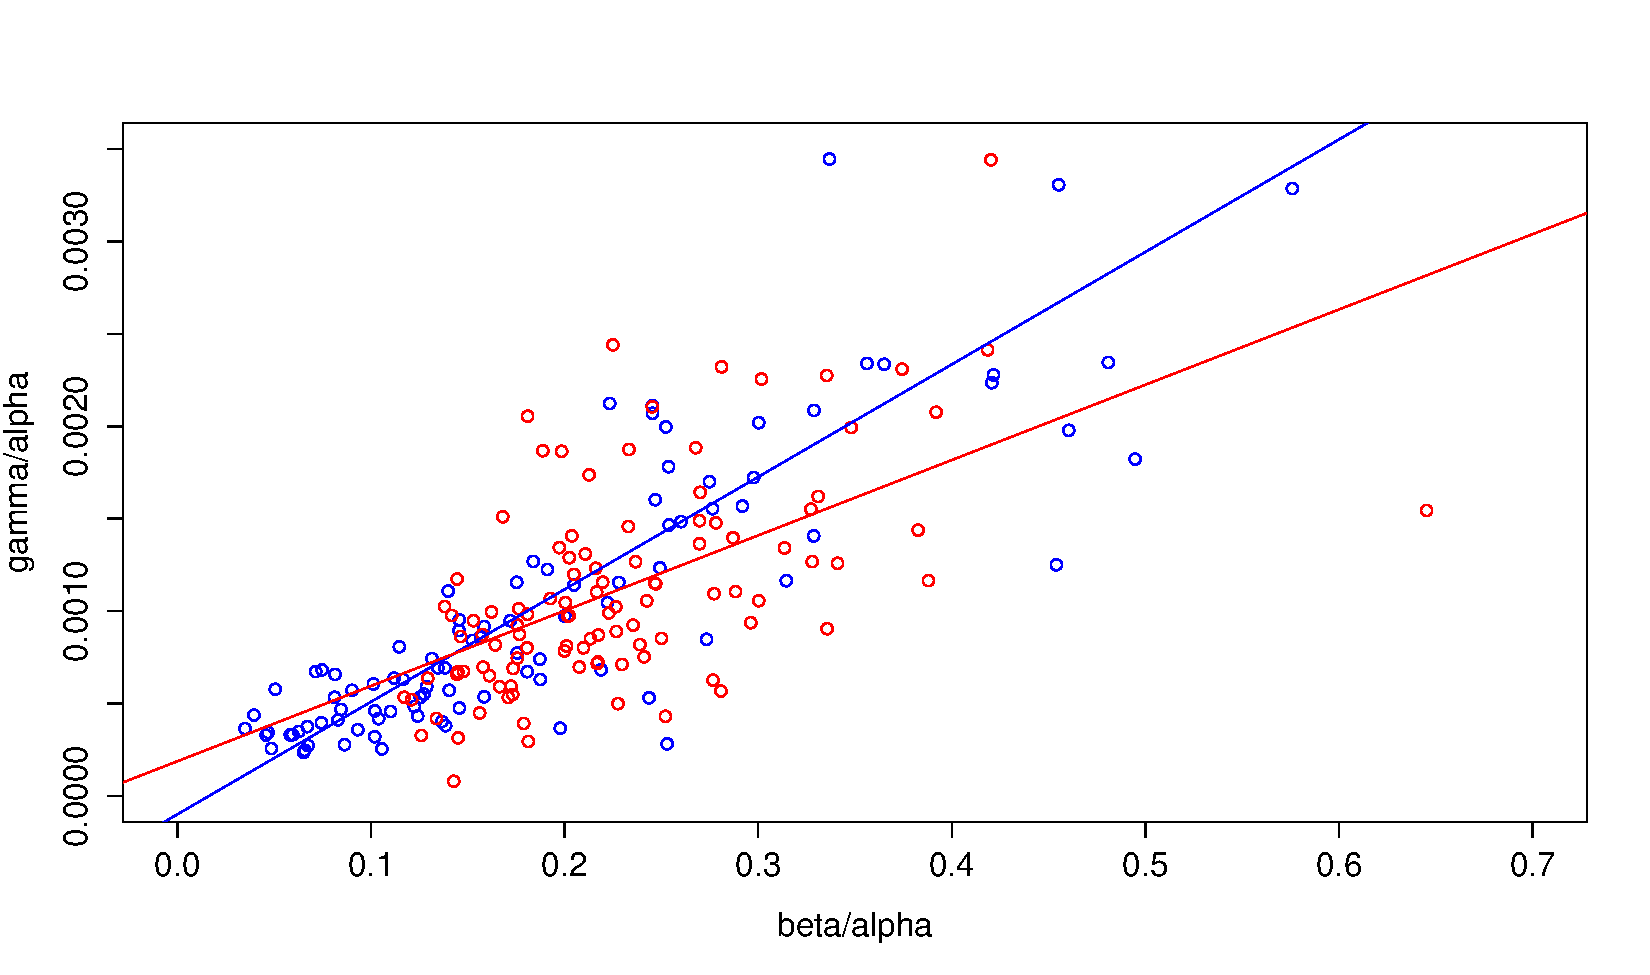
\includegraphics[width=\textwidth]{GMmaxmaj.pdf}
\label{fig:correlation}
\end{figure}

Since the variation of Grantham weights across genes is small, we set $\beta$ and $\gamma$ across all genes to be the same and optimized $g$ for each gene to get the maximum likelihood. 
Other parameters values are retained from the maximum likelihood estimates in the max approach.
We then did optimization on the common physicochemical weights $\beta$ and $\gamma$.
The ML estimates are $\beta = 0.1182$ and $\beta = 0.000574$, comparing to Grantham's weights $\beta = 0.1018$ and $\gamma = 0.000399$; and the log likelihood value is -236935.65. 
The log likelihood value increased by 2800 units comparing to the max approach when $g$ is the same across all genes. 
If other parameters including tree branch lengths and exchange rates between nucleotides are also optimized the likelihood will be increased further.
Since the number of genes is 106, allowing each gene to have different Grantham sensitivities increases the AIC value. \\

There are several reasons to explain the variation of g values between genes. 
One, these genes have different structures, which caused the different degrees of sensitivity to the difference from the optimal amino acids. 
For example, hydrophobic cores of proteins can be efficiently repacked with different hydrophobic sequences. All polar amino acids can form hydrogen bonds whose thermodynamic energy varies sharply with distance and angle, providing a rationale for the greater variability of the fitness of polar amino acids.
Two, we use the same tree topology for all genes. However, sequences in some gene might better support a different  tree topology, therefore causes other parameter estimates to be inaccurate.\\

Next we examine the g values across all 106 genes in the data by estimating all the parameters in the model separately for each gene. 
From figure \ref{fig:gvalue}, we can see that the estimates of g values under max and maj rule are consistent with max rule having a slight bigger variation. 
Figure \ref{fig:gvaluecorr} confirms the linear correlation between the estimates under the 2 approaches for finding optimal amino acids. 

\begin{figure}[h]
\caption{Plots of Grantham sensitivities across all the genes. Red are the values under max rule, and blue are under maj rule.}
\centering
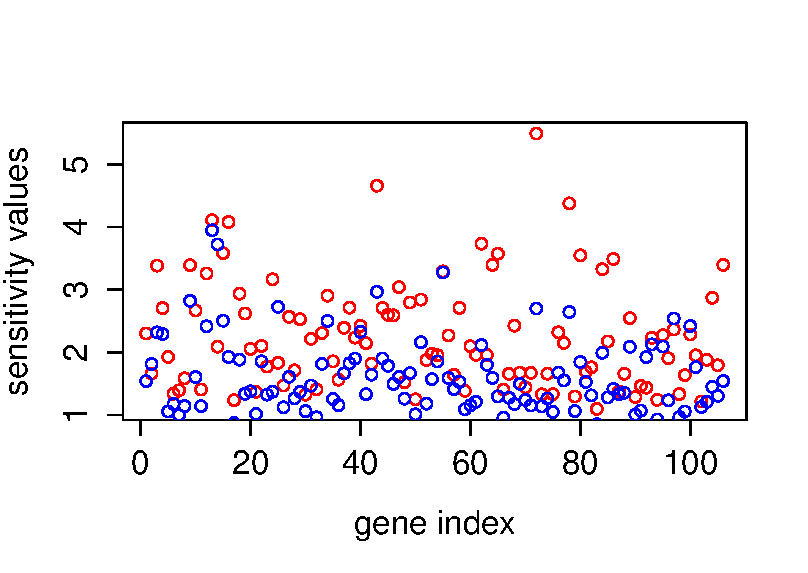
\includegraphics[width=\textwidth]{gvalue_max_maj.pdf}
\label{fig:gvalue}
\end{figure}

\begin{figure}[h]
\caption{Plots of Grantham sensitivities across all the genes. Values under max rule are plotted against under maj rule and the linear regression line is shown in red.}
\centering
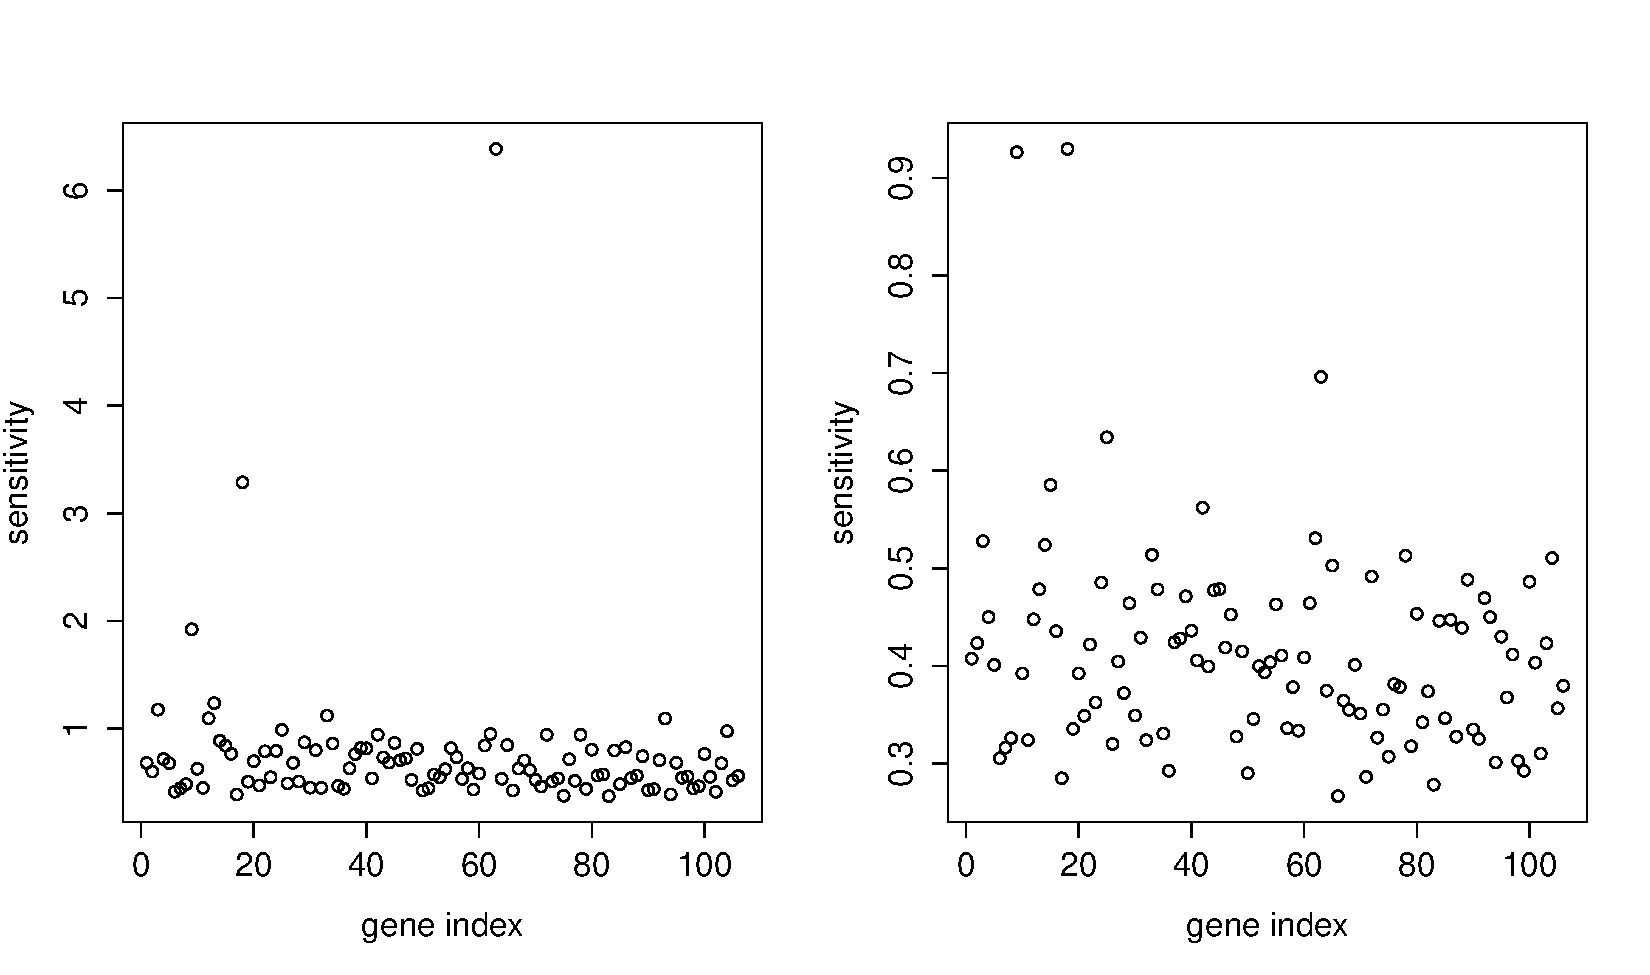
\includegraphics[width=\textwidth]{gvalue.pdf}
\label{fig:gvaluecorr}
\end{figure}


\subsubsection{Confidence of estimates of optimal amino acids}
To get the confidence level of the estimates for optimal amino acid at each site with the maximizing approach, we found the smallest set of amino acids being optimal that cover more than 95\% of the total likelihood.
In Rokas's data there are about 9000 different state patterns at the 8 species.
For each of the 9000+ sites, the likelihood values achieved by assuming each amino acid as optimal is ordered decreasingly, therefore the likelihood under the max optimal amino acid is ranked the first.
Then the next amino acid is included in the optimal set of amino acids until the total likelihood exceeds 95\% of the total likelihood.
Figure \ref{fig:AAnum} shows the histogram of numbers of optimal amino acids in the set.
The mean value for all 9000+ patterns is 5.855, and mode is 6.
The case where there are more than 10 amino acids in the set rarely happened.
Figure \ref{fig:percentile} showed the density of percentages of total likelihood value covered by the optimal amino acid found with max rule only.
Mean percentage is 0.4749 and the peak of the density distribution is between 0.3 and 0.4. (How confident are we now??)

\begin{figure}[h]
\caption{Histogram of the number of optimal amino acids together to cover at least 95\% of the total likelihood attained by all possible optimal amino acids.}
\centering
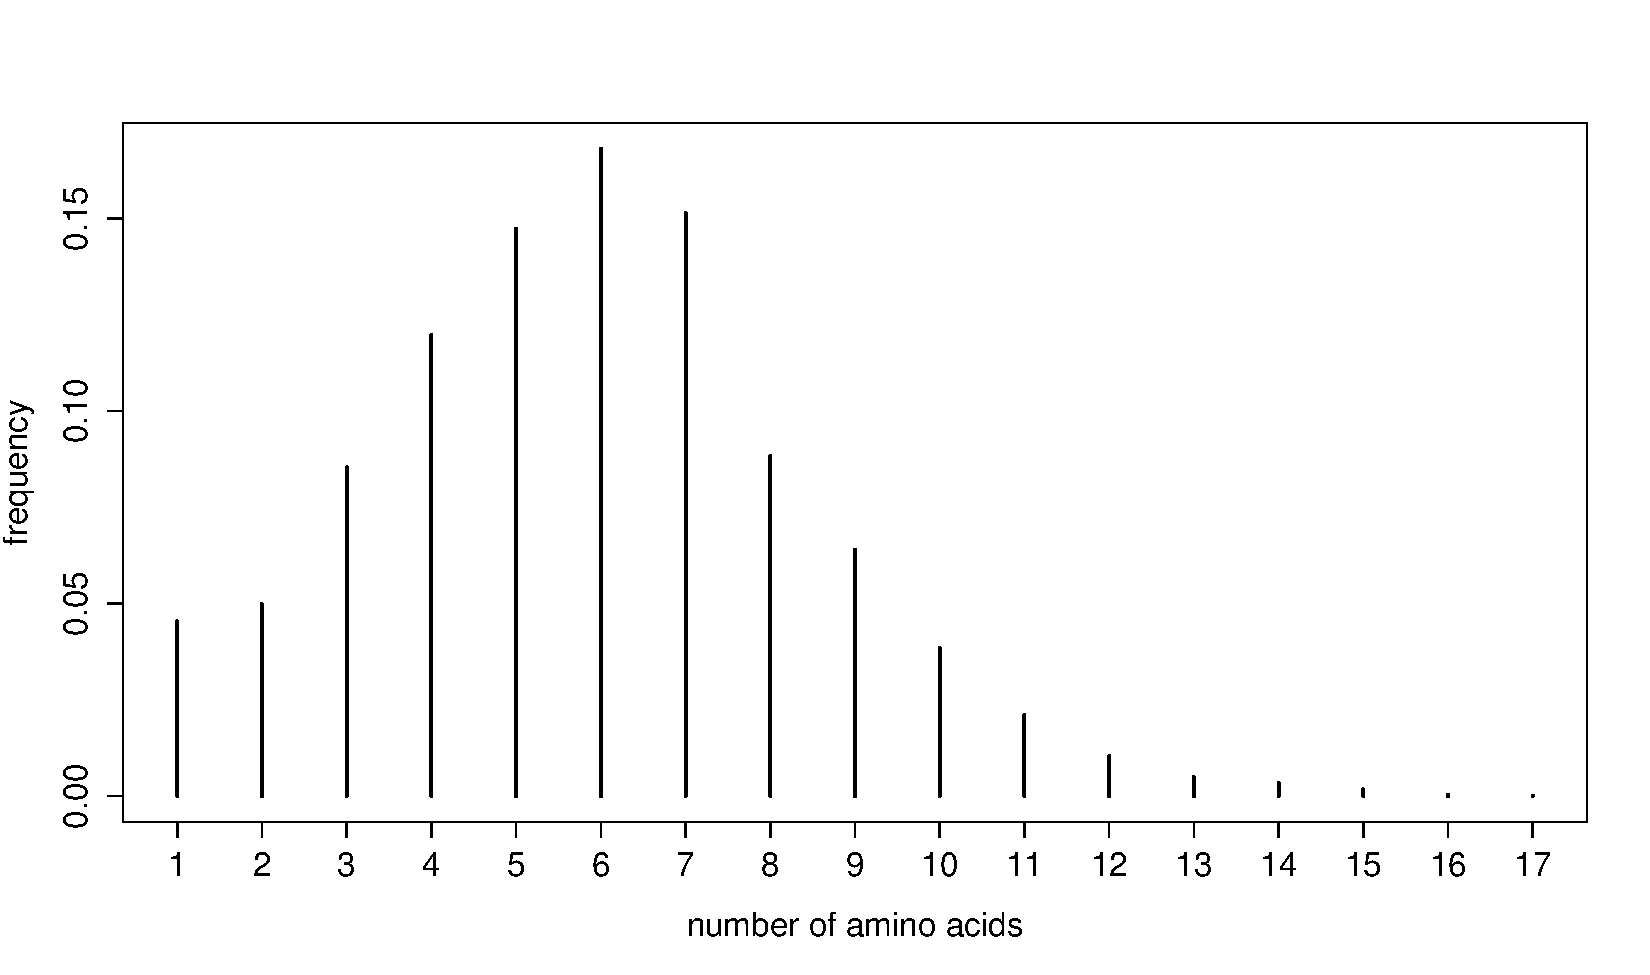
\includegraphics[width=\textwidth]{AAnum.pdf}
\label{fig:AAnum}
\end{figure}


\begin{figure}[h]
\caption{Density plot of percentages of the likelihood achieved by the optimal amino acid found by max rule.}
\centering
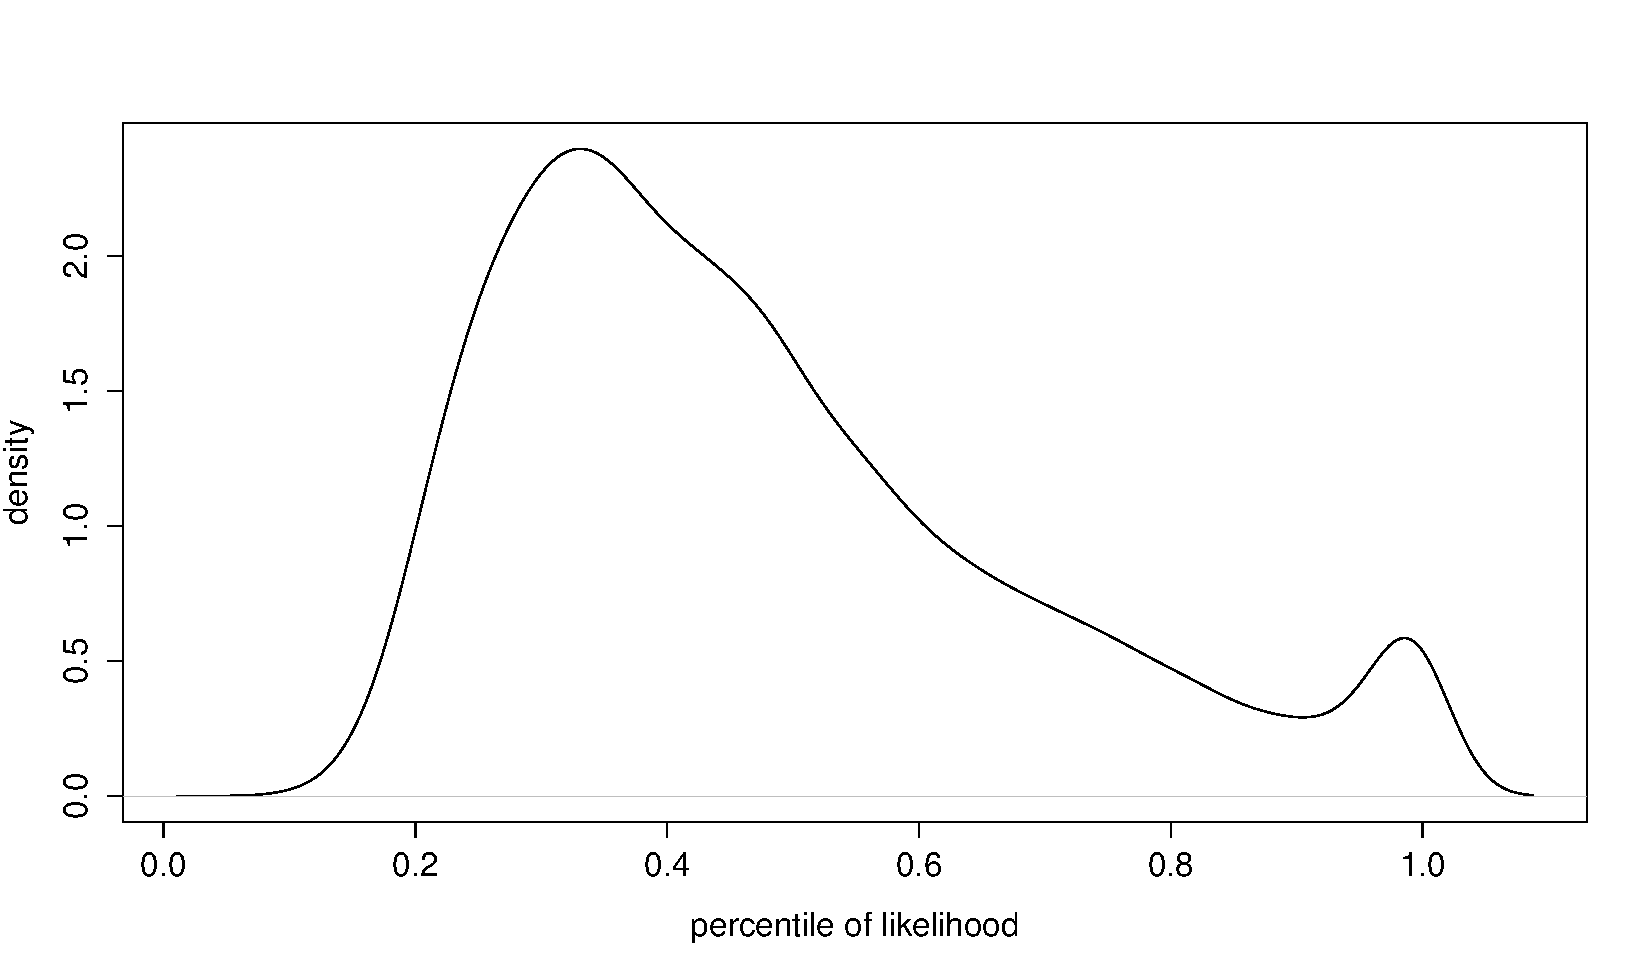
\includegraphics[width=\textwidth]{percentile.pdf}
\label{fig:percentile}
\end{figure}


%\subsubsection{Model accuracy}
%To assess model accuracy, we did simulations using the maximum likelihood estimates from Rokas et. al. 's data. (waiting on results)

\subsection{Simulated data vs. observed data}
We also evaluate the models by simulating data under models and comparing them with the observed data. 
First, a single taxon (Scas) is deleted from the Rokas's yeast gene tree, model parameters are estimated from the data on the remaining taxa. 
Then the ancestral sequence where the missing taxon is attached is estimated, where the probabilities of observing all 20 amino acids at each site are calculated. 
Then the deleted data is put back and the length of the truncated branch earlier is estimated using the parameters on the pruned tree. 
With the parameter values, the length of the missing branch, and the sequence at the start of the branch, we simulate the evolution of a gene's coding sequence from the reconstructed taxon to the deleted taxon from our analysis.
We then compare the simulated sequence at the deleted taxon with the real data. 
\begin{figure}[h]
\centering
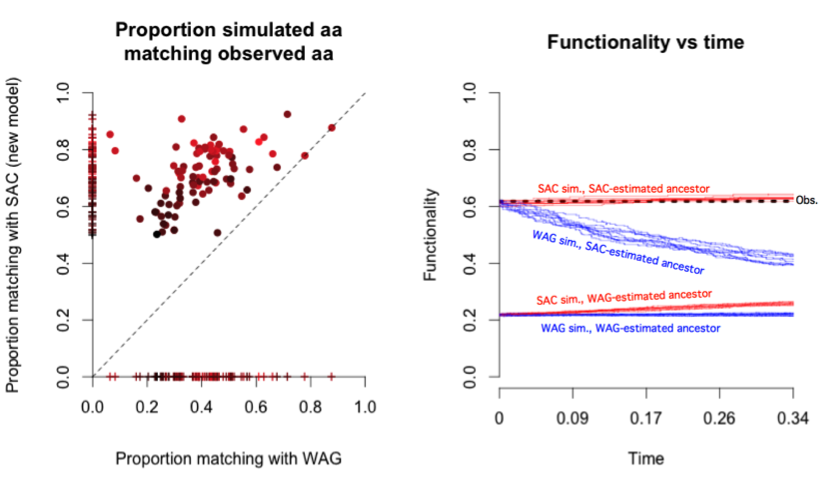
\includegraphics[width=\textwidth]{simulation.png}
\label{fig:simulation}
\end{figure}
The results are shown in Figure \ref{fig:simulation}. 
On the left, each dot represents the proportion of amino acids that differ between the simulated and the observed sequence for a given gene. 
Our new model performed much better than the standard WAG model in matching sequences, especially for genes under high selection that are shown in brighter dots. 
On the right repeated simulations are plotted under our new model (red) and WAG model (blue) starting from the ancestral sequence estimated under the estimated sequences under the new model (upper lines) and WAG model (lower lines) for a single gene. 
The dotted line represents the functionality for the observed sequence.
When the ancestral sequences are estimated from WAG model, they have much lower fitnesses. 
If evolved under WAG model, the fitness does not improve much at the end of the branch.
On the other hand there is directional selection leading to an increase in fitness if the sequences evolve under the new model. 
When the ancestral sequences are estimated from the new model the fitness is significantly higher. 
And WAG simulation leads to a decrease in fitness while the fitness is maintained under simulation with the new model.
No matter how the ancestral sequences are obtained, the new model presents a better match to the observed data.
This realistic behavior shows that the new model is more adequate than the WAG model for Rokas's data. [I THINK WE SHOULD USE THE ACTUAL BEST MODEL UNDER PROTTEST, PLUS  AA BASED ON GY94 AND GTR CODON/NUCLEOTIDE MODELS]

\end{document}